\documentclass{article}
\usepackage[version=3]{mhchem}
\usepackage{graphicx}
\usepackage{csvsimple}
\usepackage{longtable}
\usepackage{listings}
\usepackage{color} %red, green, blue, yellow, cyan, magenta, black, white
\definecolor{mygreen}{RGB}{28,172,0} % color values Red, Green, Blue
\definecolor{mylilas}{RGB}{170,55,241}
\lstset{language=Matlab,%
    %basicstyle=\color{red},
    breaklines=true,%
    morekeywords={matlab2tikz},
    keywordstyle=\color{blue},%
    morekeywords=[2]{1}, keywordstyle=[2]{\color{black}},
    identifierstyle=\color{black},%
    stringstyle=\color{mylilas},
    commentstyle=\color{mygreen},%
    showstringspaces=false,%without this there will be a symbol in the places where there is a space
    numbers=left,%
    numberstyle={\tiny \color{black}},% size of the numbers
    numbersep=9pt, % this defines how far the numbers are from the text
    emph=[1]{for,end,break},emphstyle=[1]\color{red}, %some words to emphasise
    %emph=[2]{word1,word2}, emphstyle=[2]{style},    
}
\title{%
	MATH 376: Numerical Analysis \\
	\large  Project 4: Thermocline at Platte Lake
	}
\author{Quan Vu}
\date{\today}

\begin{document}
	\maketitle
	
	\section{Abstract}
	This project investigates the thermocline, which is the horizontal plane separating regions of different temperatures in lakes. By using data, which give the depth of water and the corresponding temperature at that depth, collected at Platte Lake, we use the method of cubic spline interpolation to find a function that gives the water temperature at any given depth. Using this function and its first and second derivatives, we are able to find the position at which the thermocline occurs, and from there we can also calculate the heat flux across this thermocline.
	
	\section{Introduction}
	
	\subsection{Background information}
	In this section, we explore the method of cubic spline interpolation, which we will use to interpolate data points collected by experimentation. The data given, reflecting the various water depths and the corresponding water temperature, are collected from Platte Lake.
	
	\subsection{Problem description}
	The first task in this problem is to find a function that models water temperature with respect to changing water depths. After that, we need to find the position of the thermocline. The thermocline is defined to be the point of inflection for the temperature depth graph. In other words, this is the point where ${\frac{d^2T}{dx^2} = 0}$, where T is the temperature, measured in Celcius degrees, and x is the depth, measured in meters. Also, the thermocline is the position at which the absolute value of the first derivative of the graph is at maximum.\\
	After finding the thermocline, we determine the heat flux across the thermocline by using this equation:
	\[J = -\alpha \times \rho \times C \times \frac{dT}{dx}\]
	where ${J}$ is the heat flux in ${cal/(cm^2s}$, ${\alpha}$ is the eddy diffusion coefficient ${cm^2/s}$, ${\rho}$ is the density of water(${\approx 1 g/cm^3)}$, and ${C}$ is the specific heat of water ${\approx 1 cal/gC}$.
    
	\subsection{Outline}
	Here the method chosen to find such a function is the method of cubic spline interpolation. Since this method introduces ${3N - 3}$ unknowns, but we can only construct ${3N - 5}$ linear equations using the properties discussed in class, we have to supply ${2}$ more equations in order to find all the unknowns. The problem wants to explore natural cubic spline interpolation, meaning that if ${f(x)}$ is our function, then ${f''(x) = 0}$ at both of the outermost data points.
	
	\section{Numerical methods}
	In this project, we use the method of cubic spline interpolation, with natural endpoint conditions. Given the data points ${(x1, y1), (x2, y2), ... (xN, yN)}$, the method constructs a function that interpolates all the data points. The code to implement this is attached in the appendix.
	
	\section{Results}
    
    \subsection{Graph of temperature against depth}
    This is the graph produced by using Matlab to construct the cubic spline that interpolates all the data points given:\\
    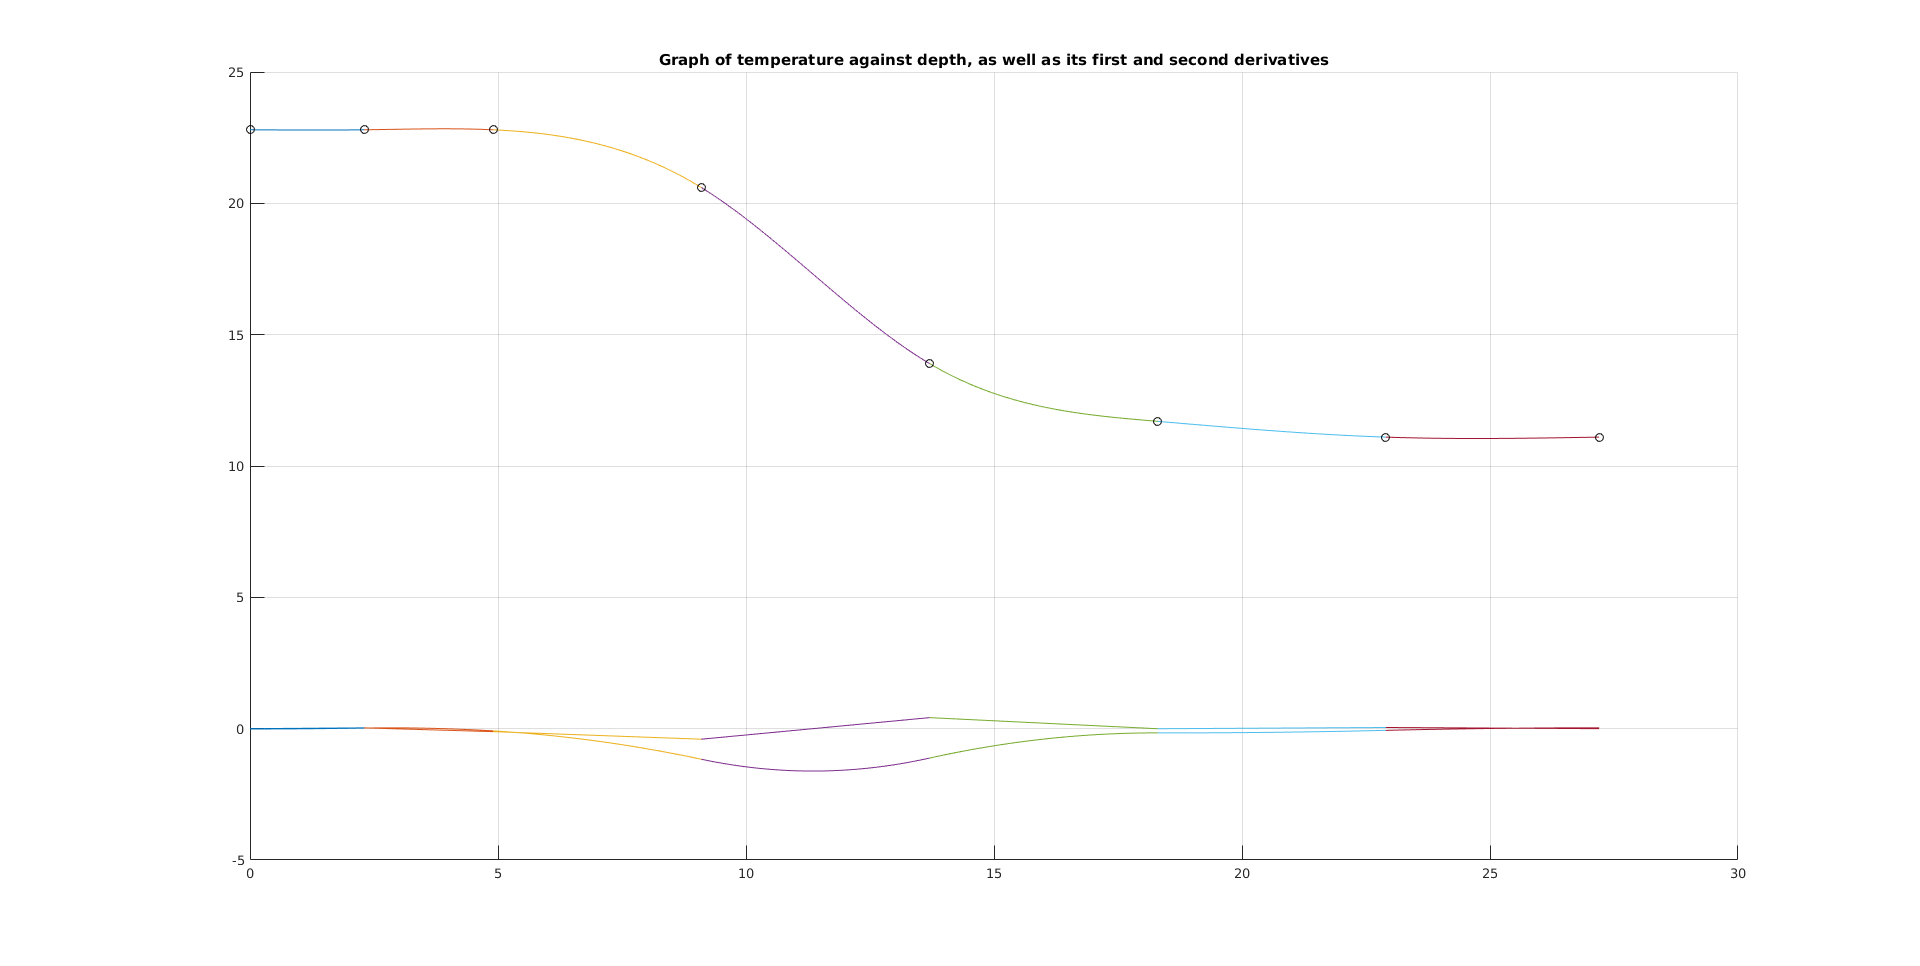
\includegraphics[scale=0.25]{Graph.png}
    \subsection{Discussion}
    From the graph given, we see that the thermocline occurs in the depth between the 4th and the 5th data points, or in the purple cubic function. We proceed to find the function modeling the temperature against depth between those 2 points using the coefficients calculated from before. The, we take the second derivative of that function with respect to the depth. After that, we use the bisection method to find the root of the second derivative in this interval, to give that the thermocline is ${\approx 11.3463673830}$. Plugging this into the equation for the heat flux, we find that the heat flux around the thermocline is ${J\approx1.614055517555187e-04}$
    \subsection{Appendix}
    \subsubsection{Natural Cubic Spline calculation in Matlab}
    \lstinputlisting{spline_natural.m}
\end{document}